\section{Background}  \label{Background}



\subsection{Autonomous Driving Systems} \label{Background:AutonomousDrivingSystems}

% thesis: Autonomous Driving Systems have high safety requirements.

Autonomous Driving Systems (ADS), defined by the Society of Automotive Engineers (SAE) as the hardware and software that are collectively capable of performing the entire dynamic driving task (DDT) on a sustained basis, should have a high safety requirements.
This term is used to describe the three most advanced Levels 3 (Conditional), 4 (High), and 5 (Full) driving automation system.

Additionally, ADS must be capable of operating under diverse operational conditions, defined as the operational design domain (ODD). The ODD includes, but is not limited to, environmental, geographical, and time-of-day conditions.
While operating under these diverse conditions, ADS can experience DDT performance-relevant system failures that prevent it from reliably performing the DDT on a sustained basis.
In such cases, the ADS must issue a request to intervene, either for the user to perform the DDT or for the system to achieve a minimal risk condition.

At Level 3, a DDT fallback-ready user is expected to take over the DDT when a DDT performance-relevant system failure occurs or when the ADS is about to leave its operational design domain (ODD). This user must be receptive and able to resume DDT performance when alerted to do so.
For example, a Level 3 ADS experiences a DDT performance-relevant system failure in one of its radar sensors, which prevents it from reliably detecting objects in the vehicle's pathway. The ADS responds by issuing a request to intervene to the DDT fallback-ready user. The ADS continues to perform the DDT, while reducing vehicle speed, for several seconds to allow time for the DDT fallback-ready user to resume operation of the vehicle in an orderly manner. It is important to highlight that a key expectation for Level 3 ADS is the capability of continuing to perform the DDT for at least several seconds after issuing the fallback-ready user with a request to intervene.

For Levels 4 and 5 ADS, if a driving automation system can perform the entire DDT and DDT fallback either within a prescribed ODD (Level 4) or in all driver-manageable on-road operating situations (Level 5), then any users present in the vehicle while the ADS is engaged are passengers. For example, if a Level 4 ADS experiences a DDT performance-relevant system failure in one of its computing modules, it transitions to DDT fallback by engaging a redundant computing module(s) to achieve a minimal risk condition.

The high safety requirements defined by SAE imply significant robustness expectations for ADS. This means that an ADS should be capable of, first, performing the DDT for a few seconds following a performance-relevant system failure until DDT fallback, and second, in the case of Levels 4 and 5, it must be able to reach a minimal risk condition despite such a system failure\cite{sae:j3016:2021apr}.

% goal: explain relevance between sensors and video object detection task

ADS should be capable of perceiving data from various sources. The DDT is defined as all real-time operational and tactical functions required to operate a vehicle in on-road traffic. Object and Event Detection and Response (OEDR) refers to the subtasks of the DDT that include monitoring the driving environment (detecting, recognizing, and classifying objects and events, and preparing to respond as needed) and executing an appropriate response to such objects and events (i.e., actions required to complete the DDT and/or DDT fallback). Performing the OEDR is necessary to complete the DDT and DDT fallback, and the capability of a Driving Automation System to handle OEDR allows it to be classified as Level 3 automation or higher. OEDR is also known as perception and a variety of computer vision tasks fall under this category, such as object detection, semantic segmentation, 3D object detection, and others.

OEDR tasks rely on exteroceptive sensors for perception hardware, which is susceptible to system failures that can compromise overall system safety. ADS system architecture is predominantly realized with two approaches: modular \cite{} or end-to-end \cite{} see Figure \ref{}. In both approaches, pipelines \cite{} start with feeding raw sensor inputs to downstream system, either localization and object detection modules or an end-to-end model. Exteroceptive sensors, mainly used for commonly employed modalities for perceiving the environment, include cameras, LiDAR (light detection and ranging), radar, and ultrasonic sensors. These sensors vary in technologies and may exhibit various failures \cite{}. The scope of this thesis will specifically investigate two critical failure modes: (1) non-deterministic sensor input availability, where the system receives inconsistent or temporally varying subsets of data from its sensors, and (2) the complete failure of a sensor component, where it provides no signal. Temporal Calibration, a mitigation strategy, establishes the synchronization rate of multiple sensor data streams \cite{}. While Temporal Calibration aims to mitigate the first failure mode of non-deterministic sensor input, it cannot rule it out completely. This limitation stems from the asynchronous publish-subscribe communication model inherent in common ADS middleware frameworks like the Robot Operating System (ROS). In such systems, message delivery times for sensor data are not strictly guaranteed and can be influenced by variable factors including network latency, system processing load, and underlying operating system scheduling priorities. Consequently, even when employing ROS tools designed for time synchronization, these inherent timing uncertainties and potential for message delays or drops mean that perfect, deterministic, real-time alignment of all sensor data streams cannot always be achieved, leaving residual non-determinism in sensor input availability. The complete sensor failure has no mitigation strategy except sensor redundancy \cite{}.

% TODO: add figure architecture

\subsection{Video Object Detection} \label{Background:VideoObjectDetection}

% Object detection definition. Deep learning pushed performance of single image object detection.

Object detection is a foundational challenge in computer vision and has been a subject of research for several decades \cite{fischlerRepresentationMatchingPictorial1973}. The goal of the object detection task is to find objects of a given description in images and videos.
Advancements in deep learning techniques for feature representation learning \cite{hintonReducingDimensionalityData2006, lecunDeepLearning2015}, coupled with the significant development and application of deep convolutional neural networks (CNNs), have driven remarkable progress in various computer vision tasks, such as image classification \cite{}, object detection \cite{} etc..
Extending detection capabilities from static images to video sequences introduces the task of video object detection (VID), which involves not only localizing objects within each frame but also leveraging temporal information across frames for improved accuracy and consistency.
The introduction of specific challenges, such as the video object detection track in the ImageNet Large Scale Visual Recognition Challenge (ILSVRC) \cite{russakovskyImageNetLargeScale2015}, provided benchmark datasets and standardized evaluation protocols, significantly accelerating research and development in the VID domain.

% State-of-the-Art
% Still-image detector
Due to the inherent similarity between detecting objects in single images and in video frames, the most straightforward approach to VID is to apply a single-image object detector independently to each frame \cite{placeholder_static_detector_for_vid}. This method, often referred to as frame-by-frame detection, treats each frame as independent image. However, such an approach ignores the rich temporal and contextual information available across consecutive video frames. Neglecting this temporal dimension often leads to suboptimal performance, characterized by issues like inconsistent bounding box predictions across frames, flickering detections, and reduced robustness to challenges specific to video, such as motion blur or partial occlusion \cite{placeholder_vid_limitations_survey}. Consequently, while applying static detectors frame-by-frame serves as a simple baseline, it is generally not considered an effective or optimal solution for the complexities of video object detection.

% Postprocessing (not e2e)

%One intuition to improve temporal consistency is to propagate detection results to neighbor frames to reduce sudden changes of detection results.

%In this work we propose a simple extension of single image object detection to help overcome these difficulties.

Video object detection methods can be broadly classified based on their architectural approaches to incorporating temporal information. A survey \cite{jiaoNewGenerationDeep2022} categorizes these techniques into several groups: including postprocessing methods, approaches introducing additional models, feature filtering mechanisms, and other effective networks.

One strategy involves applying a postprocessing step to the outputs of a still-image detector to enhance temporal consistency \cite{hanSeqNMSVideoObject2016, kangTCNNTubeletsConvolutional2018, kangObjectDetectionVideo2016}. This often utilizes detections from adjacent frames to refine results for the current frame. Common postprocessing techniques include Sequence Non-Maximum Suppression (Seq-NMS), which links high-scoring detection boxes across frames into sequences \cite{hanSeqNMSVideoObject2016}, or leveraging optical flow to propagate detection scores \cite{kangTCNNTubeletsConvolutional2018, kangObjectDetectionVideo2016, zhuFlowGuidedFeature2017}. While these methods can improve upon static image detectors, exploiting temporal information solely during postprocessing is considered suboptimal, as crucial temporal and motion cues are disregarded during the primary detector training phase.

To address the limitations of postprocessing, another category of methods utilize additional models to integrate motion and temporal information directly into the model training, often creating end-to-end solutions. Recurrent Neural Networks (RNNs) and their variants are frequently employed for this purpose. Paper \cite{Lu_2017_ICCV} proposed using a Long Short-Term Memory (LSTM) network \cite{6795963} to refine detection results by incorporating association features that represent detected objects across frames. This allows for joint, end-to-end training with the object detector. However, this specific LSTM-based association approach primarily relies on object links between adjacent frames, limiting its effectiveness in handling long-term occlusions or significant appearance changes, similar to issues faced by postprocessing methods.

Another significant RNN-based contribution is the Spatio-Temporal Memory Module (STMM) \cite{xiaoVideoObjectDetection2018}. This module utilizes a Convolutional Gated Recurrent Unit (ConvGRU) \cite{ballasDelvingDeeperConvolutional2016}, a variant of GRUs designed to preserve spatio-temporal structure within feature maps. The STMM aggregates information over time, allowing the model to leverage context from previous frames stored in its memory. Research suggests that the effectiveness of such memory modules increases with sequence length, as more relevant long-range information can be accumulated, leading to improved detection performance, particularly for objects undergoing occlusion or appearance changes. Other works also explore variants like temporally-aware feature maps integrated with ConvGRU or LSTM structures for mobile applications \cite{}.

More recently, Transformer architectures \cite{vaswaniAttentionAllYou2017} have demonstrated significant potential in computer vision tasks, including object detection \cite{carionEndToEndObjectDetection2020, zhuDeformableDETRDeformable2021}. Models like DETR (DEtection TRansformer) \cite{carionEndToEndObjectDetection2020, zhuDeformableDETRDeformable2021} and its derivatives aim to simplify the traditional detection pipeline by reformulating object detection as a set prediction problem, eliminating the need for hand-designed components like NMS or anchor generation found in many CNN-based detectors. While newer to video object detection compared to RNNs, Transformers offer a different paradigm for modeling long-range dependencies and object relationships within sequences \cite{wangEndtoEndVideoObject2021, shvetsTrackingObjectsAs2021}.

\subsection{General Purpose Perceiver Model} \label{Background:Perceiver}

Most architectures used by AI systems today are specialized. For instance, models presented in \ref{Background:VideoObjectDetection} built for the video object detection task might excel at processing 2D video frames, but they are hardly ideal for other data types, such as the LiDAR point clouds or radar output used in ADS. Handling multiple data modalities, like the sounds and images that make up videos, presents even greater complexity and usually involves complex, hand-tuned systems built from many different parts, even for simple tasks. Real-world problems, such as building an ADS, possess these complexities, so there is a desperate need to build a simple yet effective, more general, and versatile architecture that can handle all types of data.

Paper \cite{jaeglePerceiverGeneralPerception2021} introduces the Perceiver, a general-purpose architecture that is capable of processing different data types such as images, point clouds, audio, video, and, what is important, combinations of those to fuse together. The Perceiver builds upon the Transformer \cite{}, an architecture that uses an operation called "Attention" to map inputs into outputs \cite{}. While attention is simple and widely applicable, the way Transformers utilize attention can become memory expensive as the number of inputs grows. Consequently, Transformers perform well with inputs containing at most a few thousand elements, but common data forms like images and videos can easily comprise millions of elements. This fact poses a challenge to the generalist architecture: scaling the Transformer's attention operation to very large inputs without introducing domain-specific assumptions. The Perceiver addresses this by using attention to first encode the inputs into a small latent array. This latent array can then be processed further at a cost independent of the input's size, allowing the Perceiver's memory and computational needs to scale gracefully as the input size grows, even for particularly deep models. This "graceful growth" enables the Perceiver to achieve an unprecedented level of generality - it is competitive with domain-specific models on benchmarks based on images, 3D point clouds, and combined audio and images.

\begin{figure}
    \centering
    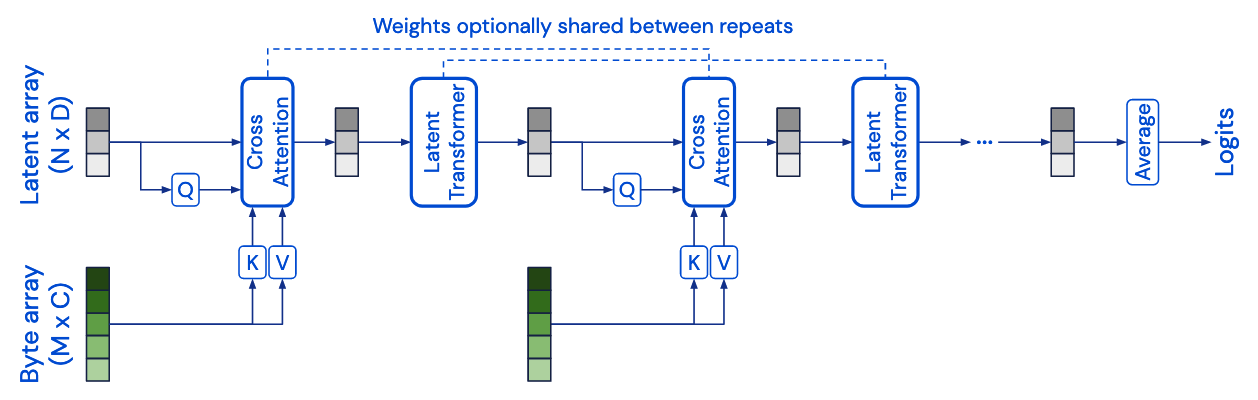
\includegraphics[width=\textwidth]{figures/figure_background_perceiver_architecture.png}
    \caption{The Perceiver is an architecture based on attentional principles that scales to high-dimensional inputs such as images, videos, audio, point-clouds, and multimodal combinations without making domain-specific assumptions. The Perceiver uses a cross-attention module to project an high-dimensional input byte array to a fixed-dimensional latent bottleneck (the number of input indices M is much larger than the number of latent indices N ) before processing it using a deep stack of Transformer-style self-attention blocks in the latent space. The Perceiver iteratively attends to the input byte array by alternating cross-attention and latent self-attention blocks \cite{jaeglePerceiverGeneralPerception2021}.}
    \label{fig:figure_background_perceiver_architecture}
\end{figure}

The Perceiver architecture is built from two components: (i) a cross-attention module that maps a byte array (e.g. an pixel array) and a latent array to a latent array, and (ii) a Transformer tower that maps a latent array to a latent array \cite{jaeglePerceiverGeneralPerception2021}. The Perceiver architecture is illustrated in Figure \ref{fig:figure_background_perceiver_architecture}. The model can be interpreted as a recurrent neural network (RNN), but unrolled in depth using the same input, rather than in time. The main challenge addressed by the architecture's design is scaling attention architectures to very large and generic inputs. The Perceiver circumvents this quadratic bottleneck through its cross-attention module. Attention is applied directly to the inputs by introducing an asymmetry into the attention operation. First, note that for $Q \in \mathbb{R}^{M \times D}$, $K \in \mathbb{R}^{M \times C}$, and $V \in \mathbb{R}^{M \times C}$, (where $C$ and $D$ are channel dimensions) the complexity of the $QKV$ attention operation - essentially, $softmax(QK^T)V$ - is $O(M^2)$, as it involves two matrix multiplications with matrices of large dimension $M$. Authors introduced asymmetry: while $K$ and $V$ are projections of the input byte array, $Q$ is a projection of a learned latent array with index dimension $N \ll M$, where the latent's index dimension $N$ is a hyperparameter. The resulting cross-attention operation has complexity $O(MN)$. This design allows Perceiver-based architectures to make use of much deeper Transformers than efficient Transformers that use linearcomplexity layers, without relying on domain-specific assumptions. This is because a Transformer built on bytes has complexity O(LM 2) while a latent Transformer has complexity O(LN 2) (where $N \ll M$), when considered as a function of the number of layers $L$ in addition to index dimensionality. The overall architecture's complexity thus becomes $O(MN + LN^2)$ for a latent Transformer with $L$ layers, and this is key: by decoupling the input size and the depth, we can add additional Transformer layers at a cost that’s independent of the input size.

However, because the original Perceiver produced only one output per input, it was not as versatile as researchers required. The Perceiver architecture is quite we want to modify it to be more like a recurrent module.